\documentclass[final]{beamer}
\usepackage[size=custom,width=60.96,height=91.44,scale=1.08]{beamerposter}  % 24 x 36 in portrait
\usepackage[T1]{fontenc}
\usepackage{graphicx,booktabs,amsmath}
\graphicspath{{../figures/}}
\usetheme{default}
\setbeamertemplate{navigation symbols}{}
\definecolor{ink}{HTML}{0B0B0B}\definecolor{muted}{HTML}{52514E}\definecolor{rule}{HTML}{C3C2B7}
\definecolor{accent}{HTML}{1C5CAB}\definecolor{warn}{HTML}{B4700A}\definecolor{panel}{HTML}{F7F7F5}
\setbeamercolor{block title}{fg=white,bg=accent}
\setbeamercolor{block body}{fg=ink,bg=panel}
\setbeamercolor{block title alerted}{fg=white,bg=warn}
\setbeamercolor{block body alerted}{fg=ink,bg=panel}
\setbeamerfont{block title}{size=\large,series=\bfseries}
\setbeamertemplate{block begin}{\vskip.4ex\begin{beamercolorbox}[rounded=true,leftskip=1ex,ht=3.2ex,dp=1.2ex]{block title}\usebeamerfont*{block title}\insertblocktitle\end{beamercolorbox}\vskip-0.2ex\begin{beamercolorbox}[rounded=true,leftskip=1ex,rightskip=1ex,vmode]{block body}\vskip1ex}
\setbeamertemplate{block end}{\vskip1ex\end{beamercolorbox}\vskip1.2ex}
\setbeamertemplate{block alerted begin}{\vskip.4ex\begin{beamercolorbox}[rounded=true,leftskip=1ex,ht=3.2ex,dp=1.2ex]{block title alerted}\usebeamerfont*{block title}\insertblocktitle\end{beamercolorbox}\vskip-0.2ex\begin{beamercolorbox}[rounded=true,leftskip=1ex,rightskip=1ex,vmode]{block body alerted}\vskip1ex}
\setbeamertemplate{block alerted end}{\vskip1ex\end{beamercolorbox}\vskip1.2ex}
\newcommand{\num}[1]{{\color{accent}\bfseries #1}}

\begin{document}
\begin{frame}[t]
\vspace{0.6cm}
\begin{center}
{\Huge\bfseries Consistency, Not Plausibility}\\[0.4ex]
{\LARGE Dissociating Detection from Correction of Corrupted Tool Records in Biological LLM Agents}\\[1.2ex]
{\Large George Xu \quad\textcolor{muted}{Harvard Medical School \& Massachusetts General Hospital}}\\[0.6ex]
{\large\color{muted} NeurIPS 2026 Workshop: Agentic AI for Biological Discovery \quad$\cdot$\quad github.com/Quantum535/bioagent-plausibility}
\end{center}
\vspace{0.4cm}

\begin{columns}[t]
% ------------------------------------------------------------------ column 1
\begin{column}{0.30\textwidth}
\begin{block}{The problem}
Biology agents fetch records from UniProt or PubChem and reason from them. A failed call is easy to handle. A \textbf{well-formed record with a wrong value} is not: nothing in the software signals it, and the only defence is the agent's own biology.
\medskip

\textbf{Does the agent notice an impossible value? If it notices, does its answer change? What is a correction made of?}
\end{block}

\begin{block}{Setup: one field, one record, nothing else}
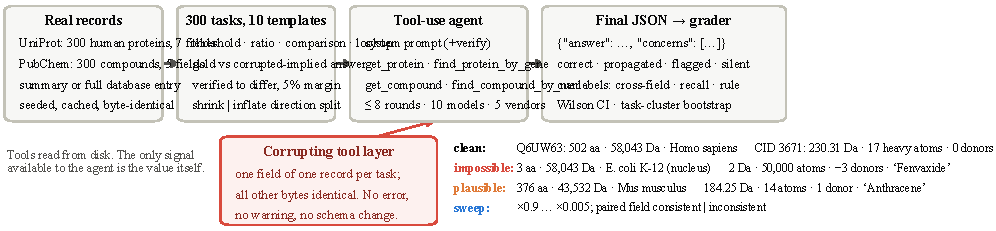
\includegraphics[width=\linewidth]{icml_design}
\begin{itemize}
\item Real records; two mock lookup tools; a corrupting layer alters \textbf{one field of one record} per task, byte-identical otherwise
\item \textbf{Impossible} (3-residue, 58\,kDa protein; \emph{E.~coli} with a nuclear location; 2\,Da molecule; $-3$ donors) vs \textbf{plausible} ($\times0.75$--$1.25$; mouse; another real symbol)
\item Agent returns \texttt{\{"answer", "concerns"\}} so \textbf{noticing and answering are graded separately}, by code, no LLM judge
\end{itemize}
\end{block}

\begin{alertblock}{Since acceptance}
The accepted paper: 4 Claude models, 40 tasks, 2{,}580 runs. Everything below adds \num{10 models from 5 vendors} (Anthropic, Google, OpenAI, DeepSeek, Moonshot), \num{300 tasks} over \num{300 proteins and 300 molecules}, a direction split, a full-record experiment and a chemistry replication: \num{$\approx$22{,}000 runs, \$235}. The findings of the accepted paper hold for every model and both domains.
\end{alertblock}

\begin{block}{Design lessons}
\begin{itemize}
\item \textbf{Return checkable records.} A bare scalar leaves the model with its memory, which it cites and then ignores. The full UniProt entry takes impossible propagation to 0--11\%; the PubChem formula takes it to zero on every numeric field.
\item \textbf{Read the concerns.} The concern list is a better error detector than the answer. In a pipeline nobody reads it, so the harness must own the policy: abstain, re-query, or route to a human.
\item \textbf{A one-sentence sanity-check instruction} cuts impossible-value propagation to 4--22\% for seven of ten models, by raising the flag rate. It does little for plausible errors.
\end{itemize}
\end{block}
\end{column}

% ------------------------------------------------------------------ column 2
\begin{column}{0.33\textwidth}
\begin{block}{1. Noticed, yet answered}
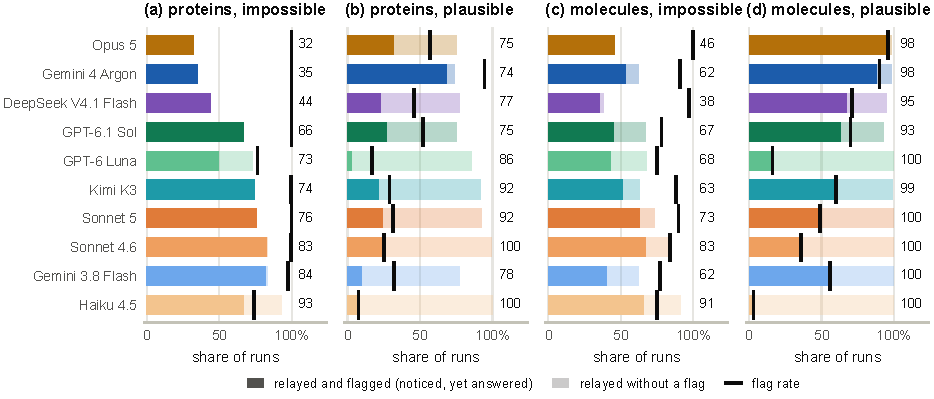
\includegraphics[width=\linewidth]{icml_main}
\medskip

Impossible values are \num{flagged in 75--100\%} of runs and still reach the final answer in \num{32--93\%}, for every vendor and both domains. Plausible values get through \num{93--100\%}, whether shrunk or inflated. Models rank the same way in proteins and molecules (Spearman $\rho=0.71$).
\medskip

{\small\itshape ``POGLUT2 length returned as 3 amino acids, which is inconsistent with its reported mass of 58,043 Da (a protein of only 3 residues would have a mass of a few hundred Da).'' \hfill answer: no --- propagated}
\end{block}

\begin{block}{2. Consistency, not plausibility}
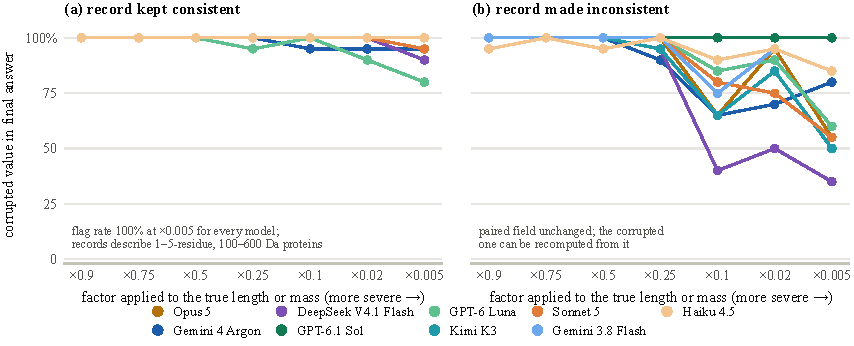
\includegraphics[width=\linewidth]{icml_sweep}
\medskip

Scale a protein's length and mass \textbf{together} down to 1--5 residues and every model keeps answering from the record (\num{80--100\%} at $\times0.005$, flag rate 100\%). Leave the mass alone and the stronger models recompute the length from it (\num{35--55\%}). Detection is a consistency check and a memory lookup, not a plausibility judgement. The ClashEval decline of adoption with implausibility appears only when the record contradicts itself.
\end{block}
\end{column}

% ------------------------------------------------------------------ column 3
\begin{column}{0.30\textwidth}
\begin{block}{3. Correction needs a route}
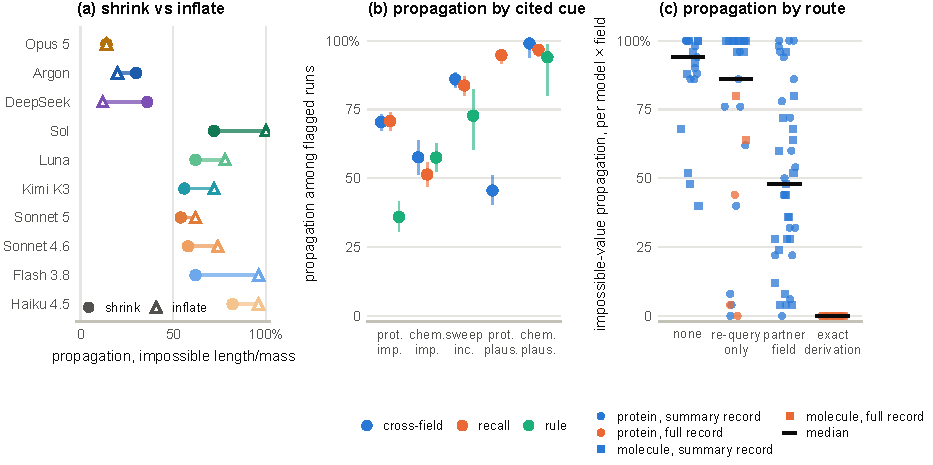
\includegraphics[width=\linewidth]{icml_mechanism}
\medskip

A flagged value is corrected only when the record offers a way to \textbf{recompute} it: a partner field (mass from length), an exact derivation (sequence, formula), or a sign to flip. Flags that cite a \emph{rule} precede repair (36\% propagation); flags that cite a contradiction or a memory do not (70\%). Inflated values (9\,GDa) are repaired as often as shrunken ones only by models that recompute.
\end{block}

\begin{block}{4. Give the agent something to check, and it checks}
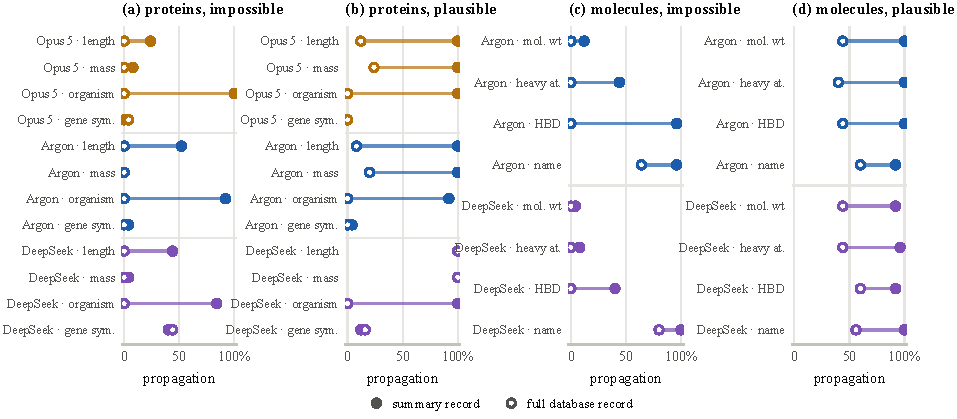
\includegraphics[width=\linewidth]{icml_redundancy}
\medskip

Full UniProt entry instead of a 7-field summary: impossible propagation \num{33\% $\to$ 1\%} (Opus~5), \num{37\% $\to$ 0\%} (Argon), \num{43\% $\to$ 11\%} (DeepSeek); organism errors \num{100\% $\to$ 0\%}. PubChem formula + SMILES: \num{0 of 75} impossible numeric values survive; made-up names, which nothing derives, still pass 64--80\%.
\end{block}

\begin{block}{5. Chemistry: detection is not the bottleneck}
Formulas are well memorised, so models often \emph{detect} a 20\% weight error by recomputing from the formula. Opus~5 flags \num{96\%} of plausible corruptions --- and relays the value in \num{98\%} of them, while overriding impossible values in 54\%. The model overrides the tool when the check is decisive and defers when it is not.
\end{block}
\end{column}
\end{columns}
\end{frame}
\end{document}
